% Options for packages loaded elsewhere
\PassOptionsToPackage{unicode}{hyperref}
\PassOptionsToPackage{hyphens}{url}
%
\documentclass[
  ignorenonframetext,
]{beamer}
\usepackage{pgfpages}
\setbeamertemplate{caption}[numbered]
\setbeamertemplate{caption label separator}{: }
\setbeamercolor{caption name}{fg=normal text.fg}
\beamertemplatenavigationsymbolsempty
% Prevent slide breaks in the middle of a paragraph
\widowpenalties 1 10000
\raggedbottom
\setbeamertemplate{part page}{
  \centering
  \begin{beamercolorbox}[sep=16pt,center]{part title}
    \usebeamerfont{part title}\insertpart\par
  \end{beamercolorbox}
}
\setbeamertemplate{section page}{
  \centering
  \begin{beamercolorbox}[sep=12pt,center]{part title}
    \usebeamerfont{section title}\insertsection\par
  \end{beamercolorbox}
}
\setbeamertemplate{subsection page}{
  \centering
  \begin{beamercolorbox}[sep=8pt,center]{part title}
    \usebeamerfont{subsection title}\insertsubsection\par
  \end{beamercolorbox}
}
\AtBeginPart{
  \frame{\partpage}
}
\AtBeginSection{
  \ifbibliography
  \else
    \frame{\sectionpage}
  \fi
}
\AtBeginSubsection{
  \frame{\subsectionpage}
}
\usepackage{amsmath,amssymb}
\usepackage{lmodern}
\usepackage{iftex}
\ifPDFTeX
  \usepackage[T1]{fontenc}
  \usepackage[utf8]{inputenc}
  \usepackage{textcomp} % provide euro and other symbols
\else % if luatex or xetex
  \usepackage{unicode-math}
  \defaultfontfeatures{Scale=MatchLowercase}
  \defaultfontfeatures[\rmfamily]{Ligatures=TeX,Scale=1}
\fi
\usetheme[]{Singapore}
\usefonttheme{serif}
% Use upquote if available, for straight quotes in verbatim environments
\IfFileExists{upquote.sty}{\usepackage{upquote}}{}
\IfFileExists{microtype.sty}{% use microtype if available
  \usepackage[]{microtype}
  \UseMicrotypeSet[protrusion]{basicmath} % disable protrusion for tt fonts
}{}
\makeatletter
\@ifundefined{KOMAClassName}{% if non-KOMA class
  \IfFileExists{parskip.sty}{%
    \usepackage{parskip}
  }{% else
    \setlength{\parindent}{0pt}
    \setlength{\parskip}{6pt plus 2pt minus 1pt}}
}{% if KOMA class
  \KOMAoptions{parskip=half}}
\makeatother
\usepackage{xcolor}
\newif\ifbibliography
\usepackage{color}
\usepackage{fancyvrb}
\newcommand{\VerbBar}{|}
\newcommand{\VERB}{\Verb[commandchars=\\\{\}]}
\DefineVerbatimEnvironment{Highlighting}{Verbatim}{commandchars=\\\{\}}
% Add ',fontsize=\small' for more characters per line
\usepackage{framed}
\definecolor{shadecolor}{RGB}{248,248,248}
\newenvironment{Shaded}{\begin{snugshade}}{\end{snugshade}}
\newcommand{\AlertTok}[1]{\textcolor[rgb]{0.94,0.16,0.16}{#1}}
\newcommand{\AnnotationTok}[1]{\textcolor[rgb]{0.56,0.35,0.01}{\textbf{\textit{#1}}}}
\newcommand{\AttributeTok}[1]{\textcolor[rgb]{0.77,0.63,0.00}{#1}}
\newcommand{\BaseNTok}[1]{\textcolor[rgb]{0.00,0.00,0.81}{#1}}
\newcommand{\BuiltInTok}[1]{#1}
\newcommand{\CharTok}[1]{\textcolor[rgb]{0.31,0.60,0.02}{#1}}
\newcommand{\CommentTok}[1]{\textcolor[rgb]{0.56,0.35,0.01}{\textit{#1}}}
\newcommand{\CommentVarTok}[1]{\textcolor[rgb]{0.56,0.35,0.01}{\textbf{\textit{#1}}}}
\newcommand{\ConstantTok}[1]{\textcolor[rgb]{0.00,0.00,0.00}{#1}}
\newcommand{\ControlFlowTok}[1]{\textcolor[rgb]{0.13,0.29,0.53}{\textbf{#1}}}
\newcommand{\DataTypeTok}[1]{\textcolor[rgb]{0.13,0.29,0.53}{#1}}
\newcommand{\DecValTok}[1]{\textcolor[rgb]{0.00,0.00,0.81}{#1}}
\newcommand{\DocumentationTok}[1]{\textcolor[rgb]{0.56,0.35,0.01}{\textbf{\textit{#1}}}}
\newcommand{\ErrorTok}[1]{\textcolor[rgb]{0.64,0.00,0.00}{\textbf{#1}}}
\newcommand{\ExtensionTok}[1]{#1}
\newcommand{\FloatTok}[1]{\textcolor[rgb]{0.00,0.00,0.81}{#1}}
\newcommand{\FunctionTok}[1]{\textcolor[rgb]{0.00,0.00,0.00}{#1}}
\newcommand{\ImportTok}[1]{#1}
\newcommand{\InformationTok}[1]{\textcolor[rgb]{0.56,0.35,0.01}{\textbf{\textit{#1}}}}
\newcommand{\KeywordTok}[1]{\textcolor[rgb]{0.13,0.29,0.53}{\textbf{#1}}}
\newcommand{\NormalTok}[1]{#1}
\newcommand{\OperatorTok}[1]{\textcolor[rgb]{0.81,0.36,0.00}{\textbf{#1}}}
\newcommand{\OtherTok}[1]{\textcolor[rgb]{0.56,0.35,0.01}{#1}}
\newcommand{\PreprocessorTok}[1]{\textcolor[rgb]{0.56,0.35,0.01}{\textit{#1}}}
\newcommand{\RegionMarkerTok}[1]{#1}
\newcommand{\SpecialCharTok}[1]{\textcolor[rgb]{0.00,0.00,0.00}{#1}}
\newcommand{\SpecialStringTok}[1]{\textcolor[rgb]{0.31,0.60,0.02}{#1}}
\newcommand{\StringTok}[1]{\textcolor[rgb]{0.31,0.60,0.02}{#1}}
\newcommand{\VariableTok}[1]{\textcolor[rgb]{0.00,0.00,0.00}{#1}}
\newcommand{\VerbatimStringTok}[1]{\textcolor[rgb]{0.31,0.60,0.02}{#1}}
\newcommand{\WarningTok}[1]{\textcolor[rgb]{0.56,0.35,0.01}{\textbf{\textit{#1}}}}
\setlength{\emergencystretch}{3em} % prevent overfull lines
\providecommand{\tightlist}{%
  \setlength{\itemsep}{0pt}\setlength{\parskip}{0pt}}
\setcounter{secnumdepth}{-\maxdimen} % remove section numbering
% handouts
\usepackage{handoutWithNotes} 
% put 3 slides on 1 page with space for notes
%\pgfpagesuselayout{3 on 1 with notes}[a4paper, border shrink=5mm]

\setbeamertemplate{navigation symbols}{}
\setbeamertemplate{footline}[page number]

% smaller space in between lines in toc
\makeatletter
\patchcmd{\beamer@sectionintoc}{\vskip1.5em}{\vskip0.5em}{}{}
\makeatother


% two columns environmnt
\newenvironment{cols}[1][]{}{}

\newenvironment{col}[1]{\begin{minipage}{#1}\ignorespaces}{%
\end{minipage}
\ifhmode\unskip\fi
\aftergroup\useignorespacesandallpars}

\def\useignorespacesandallpars#1\ignorespaces\fi{%
#1\fi\ignorespacesandallpars}

\makeatletter
\def\ignorespacesandallpars{%
  \@ifnextchar\par
    {\expandafter\ignorespacesandallpars\@gobble}%
    {}%
}
\makeatother

%% logo on first page
\titlegraphic{\centering 
\includegraphics[width=6cm]{log_ntnu.jpg}}
\ifLuaTeX
  \usepackage{selnolig}  % disable illegal ligatures
\fi
\IfFileExists{bookmark.sty}{\usepackage{bookmark}}{\usepackage{hyperref}}
\IfFileExists{xurl.sty}{\usepackage{xurl}}{} % add URL line breaks if available
\urlstyle{same} % disable monospaced font for URLs
\hypersetup{
  pdftitle={Bayesian Statistics with R-INLA - Part 2},
  pdfauthor={Sara Martino},
  hidelinks,
  pdfcreator={LaTeX via pandoc}}

\title{Bayesian Statistics with R-INLA - Part 2}
\subtitle{Geilo, January, 2023}
\author{Sara Martino}
\date{}

\begin{document}
\frame{\titlepage}

\begin{frame}{Outline}
\protect\hypertarget{outline}{}
\tableofcontents[hideallsubsections]
\end{frame}

\hypertarget{recap}{%
\section{Recap}\label{recap}}

\begin{frame}{Latent Gaussian models}
\protect\hypertarget{latent-gaussian-models}{}
Models of the kind: \[
\begin{aligned}
\theta & \sim \pi(\theta)\\
\mathbf{x}|\theta& \sim \pi(\mathbf{x}|\theta) = \mathcal{N}(0, \mathbf{Q}^{-1}(\theta))\\
\mathbf{y}|\mathbf{x},\theta & \sim \prod_i\pi(y_i|\eta_i,\theta)
\end{aligned}
\] occurs in many, seemingly unrelated, statistical models.
\end{frame}

\begin{frame}{Main Characteristics}
\protect\hypertarget{main-characteristics}{}
\begin{enumerate}
\tightlist
\item
  Latent \textbf{Gaussian} model
\item
  The latent field has a \textbf{sparse} precision matrix (Markov
  properties)
\item
  The data are conditionally independent given the latent field
\item
  The predictor is linear
\end{enumerate}
\end{frame}

\hypertarget{markov-properties}{%
\section{Markov Properties}\label{markov-properties}}

\begin{frame}{Precision Matrix}
\protect\hypertarget{precision-matrix}{}
We always talk about the precision matrix

\[
\mathbf{Q}(\theta) = \Sigma(\theta)^{-1}
\] * Interpretaion of the elements of \(\mathbf{Q}\)

\[
\begin{aligned}
\end{aligned}
\]

\begin{itemize}
\tightlist
\item
  The precision matrix gives direct information about the conditional
  independence structure of the model
\end{itemize}

\[
x_i\perp x_j|\mathbf{x}_{-ij} \iff Q_{ij} = 0
\]
\end{frame}

\begin{frame}{Example - AR1 model}
\protect\hypertarget{example---ar1-model}{}
Consider an autoregressive process of order 1 \[
\begin{aligned}
x_t &= \phi x_{t-1} + \epsilon_t, \qquad \epsilon_t = \mathcal{N}(0,1),\qquad|\phi|<1\\
x_1&\sim\mathcal{N}(0, 1/(1-\phi^2))
\end{aligned}
\] The joint distribution is: \[
\begin{aligned}
\pi(\mathbf{x}) & =  \pi(x_1)\pi(x_2|x_1)\dots\pi(x_n|x_{n-1})\\
 & = \frac{1}{(2\pi)^{n/2}}|\mathbf{Q}|^{1/2}\exp\left(-\frac{1}{2}\mathbf{x}^T\mathbf{Qx}\right)
\end{aligned}
\]
\end{frame}

\begin{frame}{Example - AR1 model}
\protect\hypertarget{example---ar1-model-1}{}
The precision matrix \(\mathbf{Q}\) is: \[
\mathbf{Q} =
\left(
  \begin{array}{ccccccc}
 1 & -\phi & & & & &\\
 -\phi & 1+\phi^2 & -\phi &&&& \\
  & & \ddots&\ddots&\ddots&&\\
 &&&&&&\\
 &&&&-\phi&1+\phi^2&-\phi\\
 &&&&&-\phi&1\\
\end{array} \right)
\] \pause The tridiagonal form is due to the fact that \(x_i\) and
\(x_j\) are conditionally independent for \(|i-j|>1\), given the rest.
\end{frame}

\begin{frame}{Example - AR1 models}
\protect\hypertarget{example---ar1-models}{}
Variance covariace function:

\[
\mathbf{\Sigma} =
\left(
  \begin{array}{ccccccc}
 1 & \phi & \phi^2& \phi^3&\dots & \dots& \phi^{n-1}\\
 \phi & 1 & \phi &\phi^2&\dots&\dots&\phi^{n-2} \\
  & & \ddots&\ddots&\ddots&&\\
 &&&&&&\\
 \phi^{n-2}&\phi^{n-3}&\dots&\dots&\phi&1&\phi\\
 \phi^{n-1}&\phi^{n-2}&\dots&\dots&\phi^2&\phi&1\\
\end{array} \right)
\]
\end{frame}

\begin{frame}{Precision Matrix}
\protect\hypertarget{precision-matrix-1}{}
There are two main advantages in using (sparse) precision matrix over
the variance/covariance matrix:

\begin{enumerate}
\tightlist
\item
  Building models through conditioning (``Hierarchical models'')
\item
  Computational
\end{enumerate}
\end{frame}

\begin{frame}{Building models through conditioning}
\protect\hypertarget{building-models-through-conditioning}{}
If

\begin{itemize}
\tightlist
\item
  \(\mathbf{x}\sim\mathcal{N}(0,\mathbf{Q}_x^{-1})\)
\item
  \(\mathbf{y}|\mathbf{x}\sim\mathcal{N}(0,\mathbf{Q}_y^{-1})\)
\end{itemize}

\pause

then

\[
 \mathbf{Q}_{(\mathbf{x},\mathbf{y})} =
        \begin{bmatrix}
            \mathbf{Q}_{x}+\mathbf{Q}_{y} & -\mathbf{Q}_{y} \\
            -\mathbf{Q}_{y} & \mathbf{Q}_{y}
        \end{bmatrix}
\] We don't get so nice expressions with Covariance matrix
\end{frame}

\begin{frame}{Computational benefits}
\protect\hypertarget{computational-benefits}{}
\begin{itemize}
\tightlist
\item
  Models we have seen gives a sparse precision matrix
\item
  These are much faster to compute with, than dense matrices
\item
  Special case: Kalman-filter algorithms
\end{itemize}

\pause

Tasks:

\begin{itemize}
\tightlist
\item
  Factorize \(\mathbf{Q}\) into \(\mathbf{Q}=\mathbf{L}\mathbf{L}^{T}\)
  (Cholesky)
\item
  Solve \(\mathbf{Q}\mathbf{x} = \mathbf{b}\),
  \(\mathbf{L}\mathbf{x}=\mathbf{b}\) or
  \(\mathbf{L}^{T}\mathbf{x} = \mathbf{b}\)
\item
  Compute \(\text{diag}(\mathbf{Q}^{-1})\)
\end{itemize}
\end{frame}

\begin{frame}{Numerical algorithms for sparse matrices: scaling
properties}
\protect\hypertarget{numerical-algorithms-for-sparse-matrices-scaling-properties}{}
Cholesky factorization of ``sparse'\,'
SPD\footnote{Symmetric and positive definite} matrix

\begin{itemize}
\tightlist
\item
  Time: \({\mathcal O}(n)\)
\item
  Space: \({\mathcal O}(n^{3/2})\)
\item
  Space-time: \({\mathcal O}(n^2)\)
\end{itemize}

\pause

This is to be compared with general \({\mathcal O}(n^{3})\) algorithm
for the Cholesky factorization of a SPD dense matrix.
\end{frame}

\begin{frame}{Gaussian Markov random fields}
\protect\hypertarget{gaussian-markov-random-fields}{}
\begin{itemize}
\item
  Gaussians with a sparse precision matrix are called
  \emph{Gaussian Markov random fields} (GMRFs)
\item
  Good computational properties through numerical algorithms for sparse
  matrices
\item
  Very useful for doing MCMC-based inference as well
\end{itemize}
\end{frame}

\begin{frame}{Summary}
\protect\hypertarget{summary}{}
Three main ingredients in INLA

\begin{itemize}
\item
  Gaussian Markov random fields
\item
  Latent Gaussian models
\item
  Laplace approximations

  \pause
\end{itemize}

which together (and ++++\ldots) gives a very very nice tool for Bayesian
inference:

\begin{itemize}
\tightlist
\item
  quick
\item
  accurate (relative error)
\item
  good scaling properties
\item
  +++
\end{itemize}
\end{frame}

\hypertarget{deterministic-inference-for-gaussian-models}{%
\section{Deterministic inference for Gaussian
models}\label{deterministic-inference-for-gaussian-models}}

\begin{frame}{Computations}
\protect\hypertarget{computations}{}
\Large

\hfill\break
\hfill\break
So\ldots{}\\
\strut \\
Now we have a modelling framework\ldots{}\\
\strut \\
But how do we get our answers? \normalsize
\end{frame}

\begin{frame}{What do we care about?}
\protect\hypertarget{what-do-we-care-about}{}
\textcolor{red}{It depends on the problem!}

\begin{itemize}[<+->]
\tightlist
\item
  A single element of the latent field (e.g.the sign or quantiles of a
  fixed effect)
\item
  A linear combination of elements from the latent field (the average
  over an area of a spatial effect, the difference of two effects)
\item
  A single hyperparameter (the correlation)
\item
  A non-linear combination of hyper parameters (animal models)
\item
  Predictions at unobserved locations
\end{itemize}
\end{frame}

\begin{frame}{What do we care about?}
\protect\hypertarget{what-do-we-care-about-1}{}
The most important quantity in Bayesian statistics is
\textcolor{red}{the posterior distribution}: \[
\begin{aligned}
\overbrace{\pi(\mathbf{x}, {\theta}\mid\mathbf{y})}^{{\text{Posterior}}} &\propto \overbrace{\pi({\theta}) \pi(\mathbf{x}\mid{\theta})}^{{\text{Prior}}} \overbrace{\prod_{i \in \mathcal{I}}\pi(y_i \mid x_i, {\theta})}^{{\text{Likelihood}}}
\end{aligned}
\] from which we can derive the quantities of interest, such as \[
    \begin{aligned}
        {\pi(x_i \mid \mathbf{y})} &\propto \int \int \pi(\mathbf{x}, {\theta}\mid\mathbf{y}) d{x}_{-i} d{\theta}\\
        &= {\int \pi(x_i \mid {\theta}, \mathbf{y}) \pi({\theta} \mid \mathbf{y}) d{\theta}}
    \end{aligned}
\] or \(\pi(\theta_j\mid \mathbf{y})\).

These are very high dimensional integrals and are typically not
analytically tractable.
\end{frame}

\begin{frame}{Traditional approach: MCMC}
\protect\hypertarget{traditional-approach-mcmc}{}
MCMC is based on sampling with the goal to
\textcolor{red}{construct a Markov chain with the target posterior as stationary distribution}.

\begin{itemize}
\tightlist
\item
  Extensively used within Bayesian inference since the 1980's.
\item
  Flexible and general, sometimes the only thing we can do!
\item
  A generic tool is available with \texttt{JAGS}/\texttt{OpenBUGS}.
\item
  Tools for specific models are of course available,
  e.g.\textasciitilde{}\texttt{BayesX} and \texttt{stan}.
\item
  Standard MCMC sampler are generally easy-ish to program and are in
  fact implemented in readily available software
\item
  However, depending on the complexity of the problem, their efficiency
  might be limited.
\end{itemize}
\end{frame}

\begin{frame}{Approximate inference}
\protect\hypertarget{approximate-inference}{}
Bayesian inference can (almost) never be done exactly. Some form of
approximation must always be done.

\begin{itemize}
\tightlist
\item
  MCMC ``works'\,' for everything, but it can be incredibly slow
\item
  Is it possible to make a quicker, more specialized inference scheme
  which only needs to work for this limited class of models?
  (specifically LGM)
\end{itemize}
\end{frame}

\begin{frame}{Recall: What is our model framework?}
\protect\hypertarget{recall-what-is-our-model-framework}{}
Latent Gaussian models

\[
\begin{aligned}
y| x, \theta & \sim \prod  \pi(y_i|x_i,\theta) & \\
x|\theta & \sim\mathcal{N}(0,Q(\theta)) & \text{\textcolor{red}{Gaussian!!!}}\\
\theta & \sim\pi(\theta)& \text{Not Gaussian}
\end{aligned}
\]

where the precision matrix \(Q(\theta)\) is sparse. Generally these
``sparse'\,' Gaussian distributions are called
\textcolor{red}{Gaussian Markov random fields} (GMRFs).

The sparseness can be exploited for very quick computations for the
Gaussian part of the model through numerical algorithms for sparse
matrices.
\end{frame}

\begin{frame}{The INLA idea}
\protect\hypertarget{the-inla-idea}{}
Use the properties of the LGM we have defined to approximate the
posterior \textcolor{red}{marginals}

\[
\begin{aligned}
        \pi(x_i \mid \boldsymbol{y})\quad \text{and} \quad \pi(\theta_j \mid \boldsymbol{y})
    \end{aligned}
\] directly.\\
\strut \\
Let us consider a \textcolor{red}{toy example to illustrate the ideas}.
\end{frame}

\begin{frame}{How does INLA work? A toy example}
\protect\hypertarget{how-does-inla-work-a-toy-example}{}
Smoothing noisy observations - Data

We observe some smooth function but our measures are noisy (but we know
the size of such noise!)

\begin{center}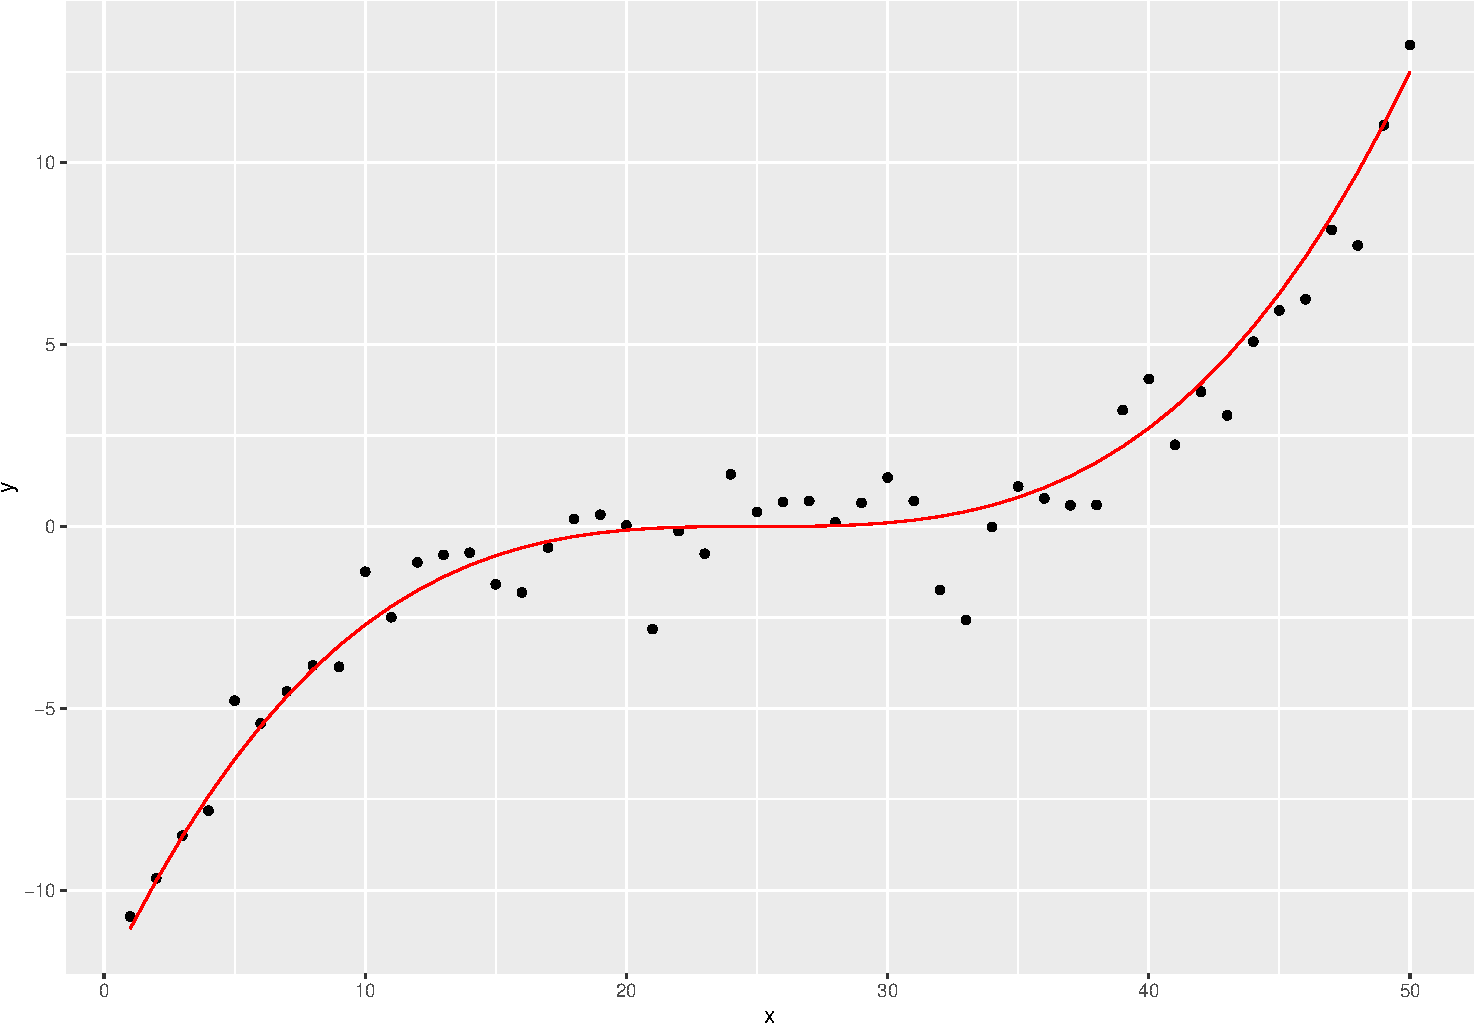
\includegraphics[width=0.6\linewidth]{Part2_deterministic_files/figure-beamer/unnamed-chunk-1-1} \end{center}

\textbf{Goal:} Recover the smooth function observed with noise!
\end{frame}

\begin{frame}{Smoothing noisy observations - Model}
\protect\hypertarget{smoothing-noisy-observations---model}{}
Assume: \begin{align*}
y_i &= f(i) + \epsilon_i; i = 1,\dots,n \\\nonumber
\epsilon_i&\sim N(0,1) \\\nonumber
f(i) &= x_i\text{ smooth function of } i\nonumber
\end{align*}

\begin{itemize}
\item
  Only one hyperparameter
\item
  Gaussian likelihood
\end{itemize}

\textcolor{red}{Is this a Latent Gaussian model?}
\end{frame}

\begin{frame}{Smoothing noisy observations - LGM}
\protect\hypertarget{smoothing-noisy-observations---lgm}{}
\begin{itemize}
\item
  \textbf{Data} Gaussian Observations with known precision \[
    y_i|x_i\sim\mathcal{N}(x_i,1)
  \]
\item
  \textbf{Latent Model}: A Gaussian model for the smooth function (RW2
  model) \[
    \pi({\mathbf x}|\theta)\propto \theta^{(n-2)/n}\exp\left\{
    -\frac{\theta}{2}\sum_{i=2}^n(x_i-2x_{i-1}+x_{i-2})^2
    \right\}
  \]
\item
  \textbf{Hyperparameter} The precision of the smooth function
  \(\theta\). We assign a Gamma prior
\end{itemize}

\[
    \pi(\theta)\propto\theta^{a-1}\exp(-b\theta)
\]
\end{frame}

\begin{frame}{Smoothing noisy observations - Goal}
\protect\hypertarget{smoothing-noisy-observations---goal}{}
Find approximations for:

\begin{enumerate}
\tightlist
\item
  The posterior marginal for the hyperparameter
  \(\pi(\theta|\mathbf{y})\)
\item
  The posterior marginals for the elements of the latent field
  \(\pi(x_i|\mathbf{y})\)
\end{enumerate}
\end{frame}

\begin{frame}{Approximating \(\pi(\theta|\mathbf{y})\)}
\protect\hypertarget{approximating-pithetamathbfy}{}
We have that \[
\pi(\mathbf{x},\theta,\mathbf{y}) = \pi(\mathbf{x}|\theta,\mathbf{y})\pi(\theta|\mathbf{y})\pi(\mathbf{y})
\]

so

\[
    \pi(\theta|\mathbf{y}) = \frac{\pi(\mathbf{x},\theta,\mathbf{y})}{\pi(\mathbf{x}|\theta,\mathbf{y})\pi(\mathbf{y})} \propto\frac{
  \pi(\mathbf{y}, \mathbf{x}|\theta)\  \pi(\theta)
    }{\pi(\mathbf{x}|\theta,\mathbf{y})}
\]

\pause

Since the likelihood is Gaussian, then
\(\pi(\mathbf{y}, \mathbf{x}|\theta)\) is also Gaussian. We have then:

\[
   \pi(\theta|\mathbf{y})  \propto \frac{
  \overbrace{\pi(\mathbf{y}, \mathbf{x}|\theta)}^{\text{Gaussian}}\  \pi(\theta)}
  {\underbrace{\pi(\mathbf{x}|\theta,\mathbf{y})}_{\text{Gaussian}}}
\] This is valid for any \(\mathbf{x}\)
\end{frame}

\begin{frame}{Posterior marginal for the hyperparameter}
\protect\hypertarget{posterior-marginal-for-the-hyperparameter}{}
Select a grid of points to represent the density
\(\pi(\theta|\mathbf{x})\)

\begin{center}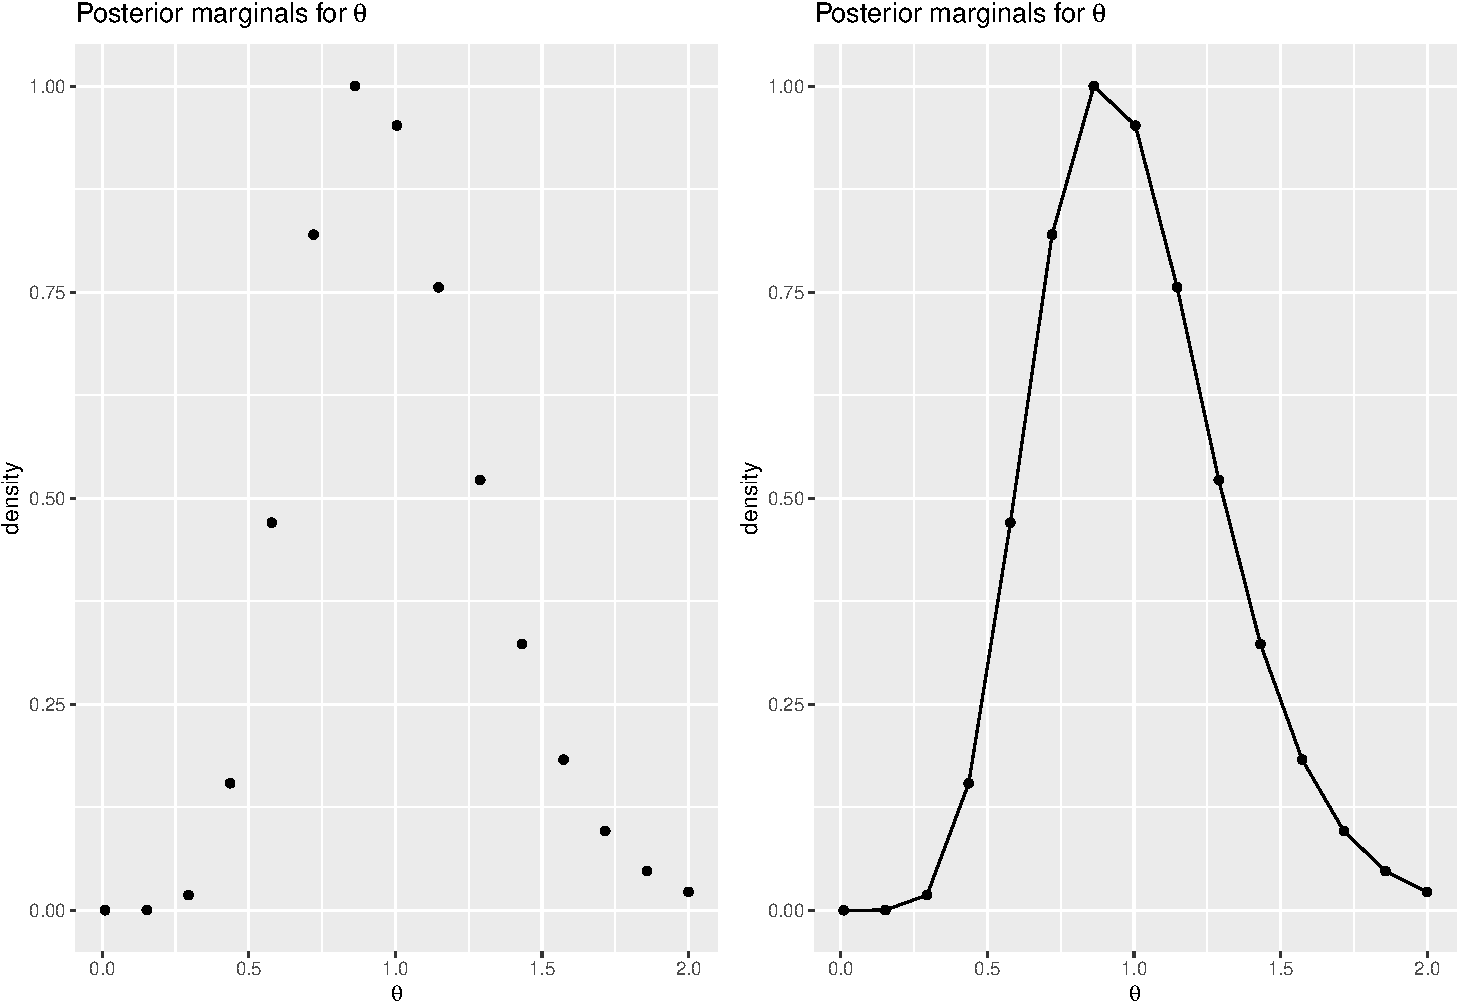
\includegraphics[width=0.6\linewidth]{Part2_deterministic_files/figure-beamer/unnamed-chunk-2-1} \end{center}
\end{frame}

\begin{frame}{Approximating \(\pi(x_i|y,\theta)\)}
\protect\hypertarget{approximating-pix_iytheta}{}
Again we have that \[
    \mathbf{x},\mathbf{y}|\theta\sim\mathbf{N}(\cdot,\cdot)
\] so also \(\pi(x_i|\theta,\mathbf{y})\) is Gaussian!!\\

We compute \begin{align*}
\pi(x_i|{\mathbf y}) &= \int \pi(x_i|\theta,{\mathbf y})\pi(\theta|{\mathbf y})d\theta\\
      &\approx \sum_k\pi(x_i|\theta_k,{\mathbf y})\pi(\theta_k|{\mathbf y}) \Delta_k
\end{align*} where \(\theta_k,k=1,\dots,K\) are the representative
points of \(\pi(\theta|\mathbf{y})\) and \(\Delta_k\) are the
corresponding weights
\end{frame}

\begin{frame}{Posterior marginals for latent field I}
\protect\hypertarget{posterior-marginals-for-latent-field-i}{}
Compute the conditional posterior marginal for \(x_i\) given each
\(\theta_k\)\\

\begin{center}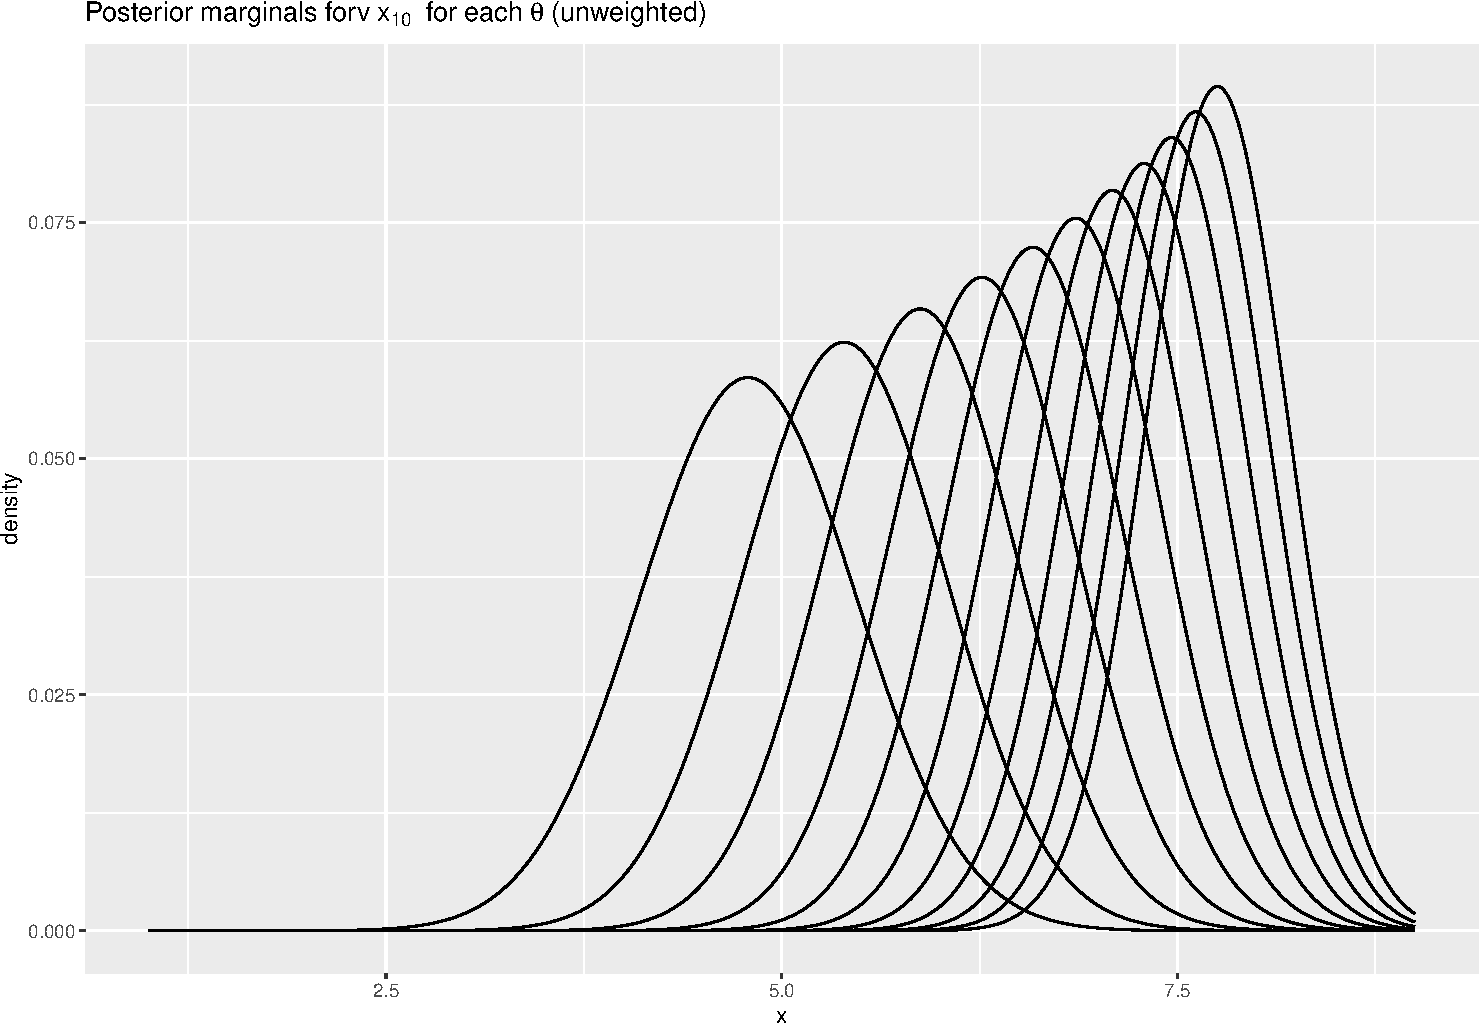
\includegraphics[width=0.6\linewidth]{Part2_deterministic_files/figure-beamer/unnamed-chunk-3-1} \end{center}
\end{frame}

\begin{frame}{Posterior marginals for latent field II}
\protect\hypertarget{posterior-marginals-for-latent-field-ii}{}
Weight the conditional posterior marginal for
\(\pi(x_i|\theta_k, \mathbf{y})\) by
\(\pi(\theta_k|\mathbf{y})\Delta_k\)

\begin{center}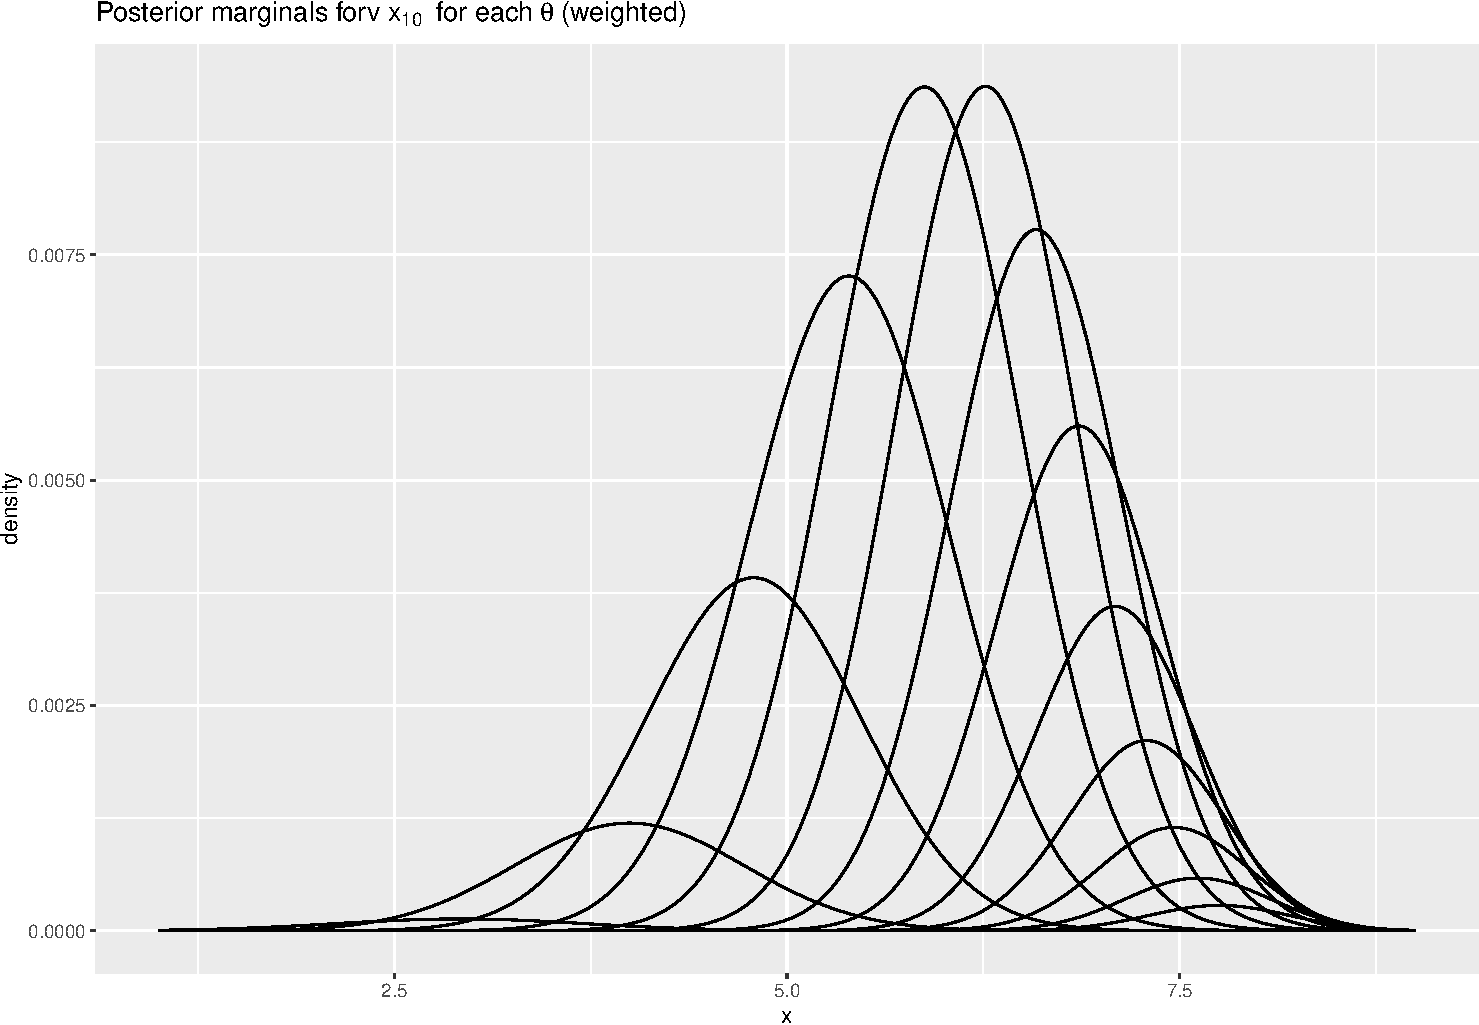
\includegraphics[width=0.6\linewidth]{Part2_deterministic_files/figure-beamer/unnamed-chunk-4-1} \end{center}
\end{frame}

\begin{frame}{Posterior marginals for latent field III}
\protect\hypertarget{posterior-marginals-for-latent-field-iii}{}
Sum to get the posterior marginal for \(x_i|\mathbf{y}\)

\begin{center}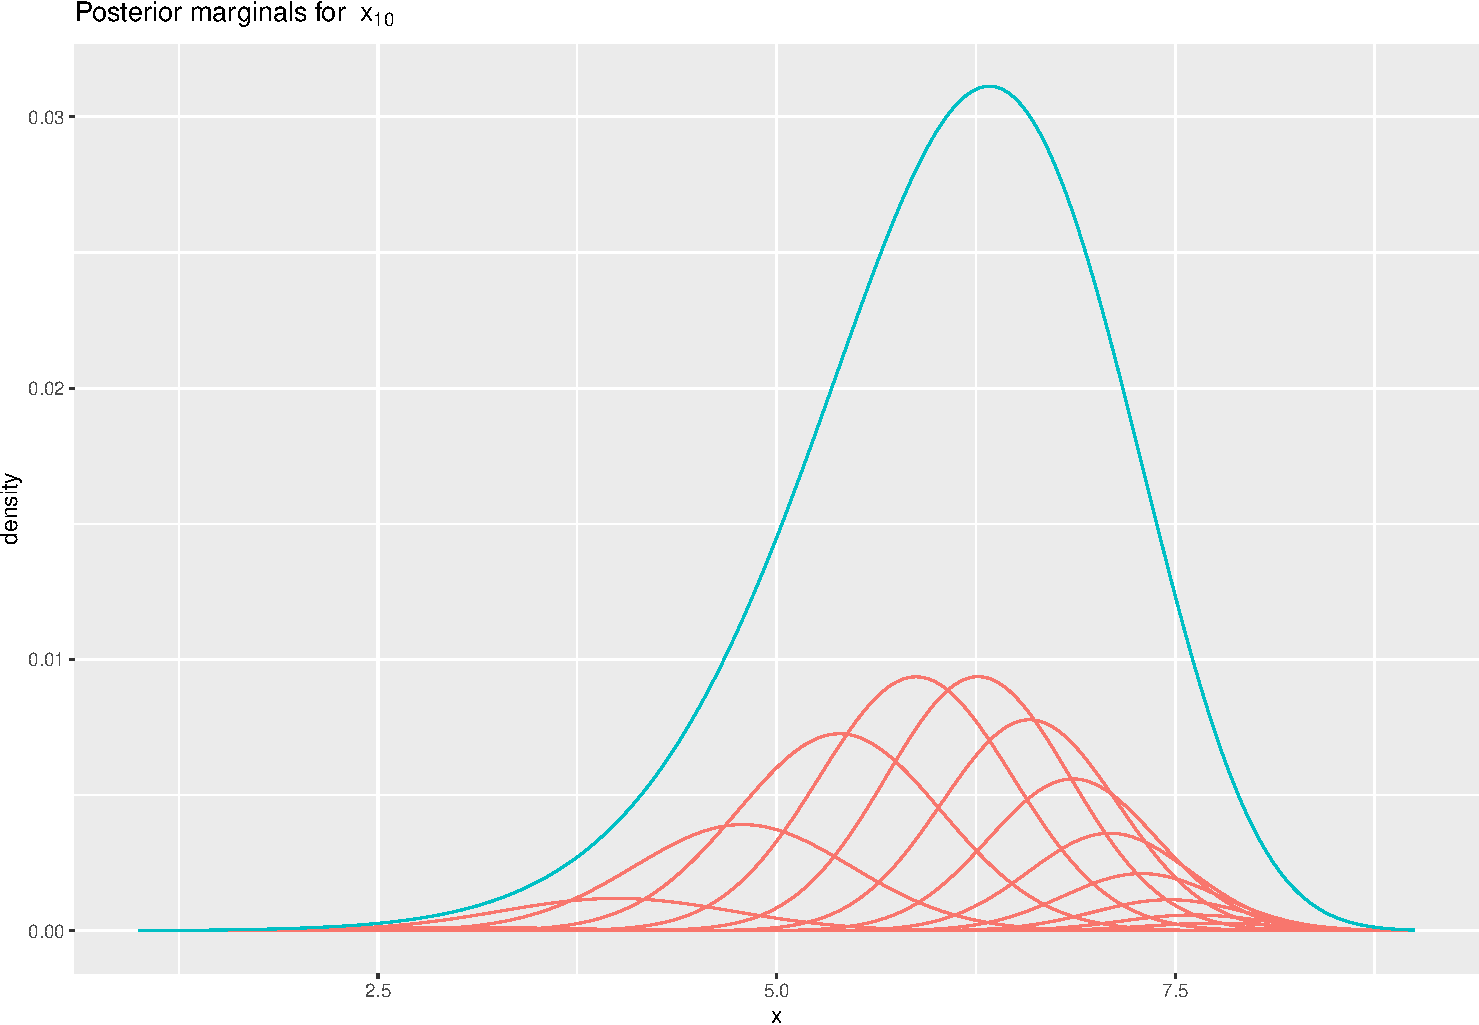
\includegraphics[width=0.6\linewidth]{Part2_deterministic_files/figure-beamer/unnamed-chunk-5-1} \end{center}
\end{frame}

\begin{frame}{Fitted Spline}
\protect\hypertarget{fitted-spline}{}
The posterior marginals are used to calculate summary statistics, like
means, variances and credible intervals:

\begin{center}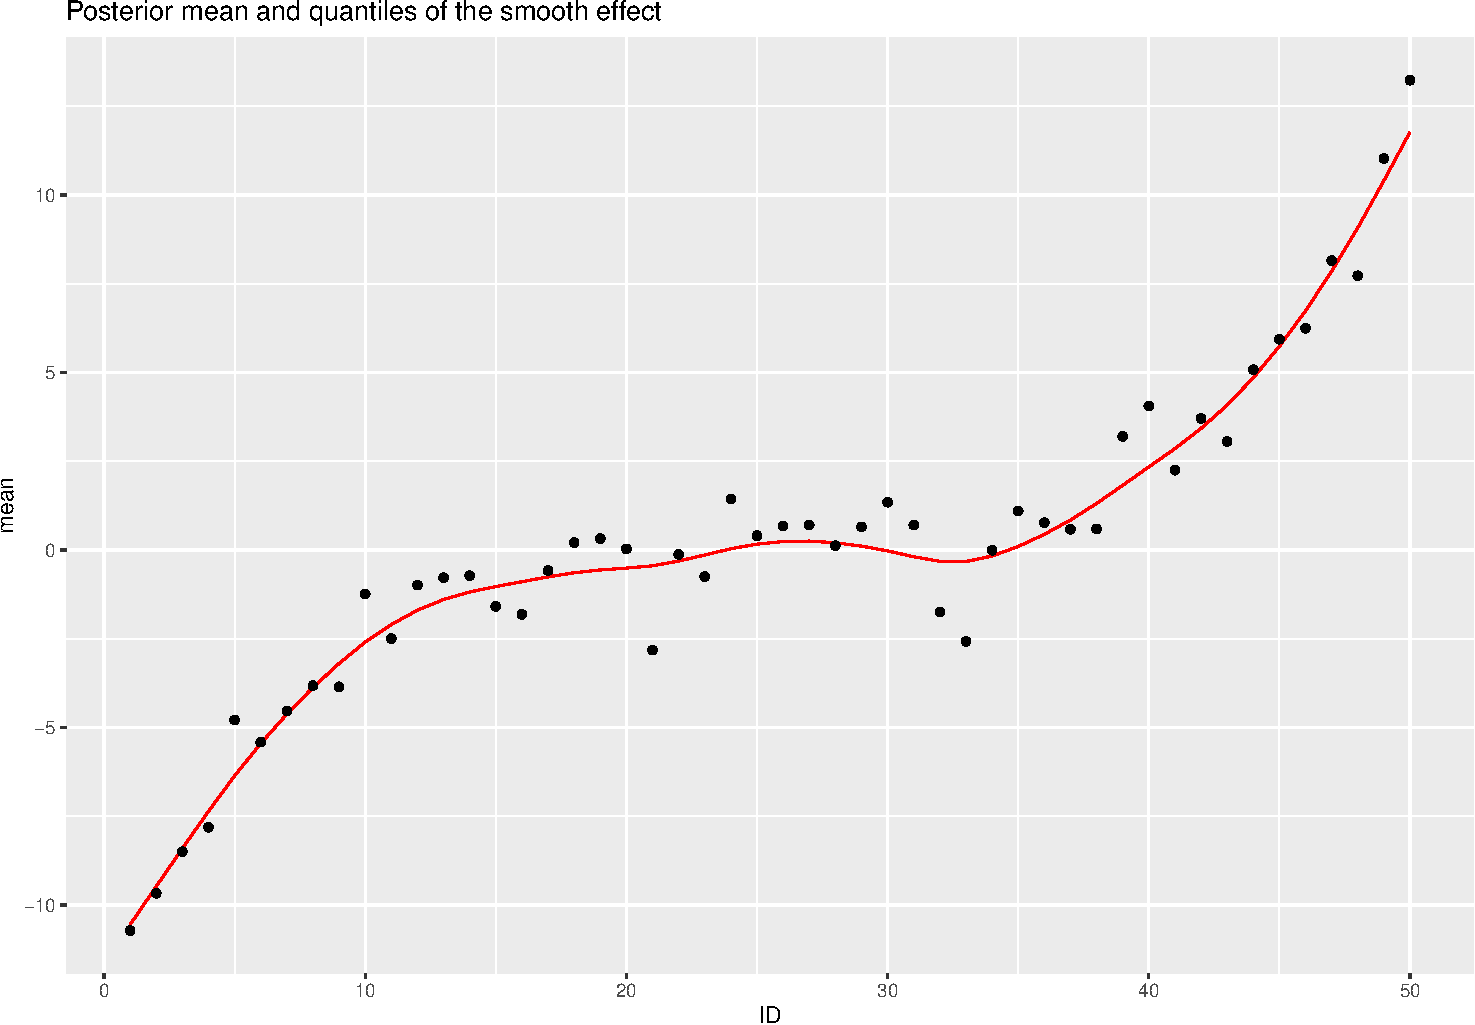
\includegraphics[width=0.6\linewidth]{Part2_deterministic_files/figure-beamer/unnamed-chunk-6-1} \end{center}
\end{frame}

\begin{frame}[fragile]{\texttt{R-INLA} code}
\protect\hypertarget{r-inla-code}{}
\small

\begin{Shaded}
\begin{Highlighting}[]
\NormalTok{formula }\OtherTok{=}\NormalTok{ y }\SpecialCharTok{\textasciitilde{}} \SpecialCharTok{{-}}\DecValTok{1} \SpecialCharTok{+} \FunctionTok{f}\NormalTok{(idx, }\AttributeTok{model=}\StringTok{"rw2"}\NormalTok{, }\AttributeTok{constr=}\ConstantTok{FALSE}\NormalTok{,}
   \AttributeTok{hyper=}\FunctionTok{list}\NormalTok{(}\AttributeTok{prec=}\FunctionTok{list}\NormalTok{(}\AttributeTok{prior=}\StringTok{"loggamma"}\NormalTok{, }\AttributeTok{param=}\FunctionTok{c}\NormalTok{(a,b))))}

\NormalTok{result }\OtherTok{=} \FunctionTok{inla}\NormalTok{(formula,}
      \AttributeTok{data =} \FunctionTok{data.frame}\NormalTok{(}\AttributeTok{y=}\NormalTok{y, }\AttributeTok{idx=}\NormalTok{idx),}
      \AttributeTok{control.family =} \FunctionTok{list}\NormalTok{(}\AttributeTok{initial =} \FunctionTok{log}\NormalTok{(tau\_0), }\AttributeTok{fixed=}\ConstantTok{TRUE}\NormalTok{))}
\end{Highlighting}
\end{Shaded}

\normalsize

This exercise is contained in the
\texttt{01\_Practical\_implement\_INLA.html} file.
\end{frame}

\hypertarget{extending-the-method}{%
\section{Extending the method}\label{extending-the-method}}

\begin{frame}{Extending the method}
\protect\hypertarget{extending-the-method-1}{}
This is the basic idea behind INLA. It is quite simple.

However, we need to extend this basic idea so we can deal with

\begin{enumerate}
\item
  Non-Gaussian observations
\item
  More than one hyperparameter
\end{enumerate}
\end{frame}

\begin{frame}{1. More than one hyperparameter}
\protect\hypertarget{more-than-one-hyperparameter}{}
\textcolor{red}{Main use:} Select good evaluation points \({\theta}_k\)
for the numerical integration when approximating
\(\widetilde{\pi}(x_i|{y})\)

\begin{itemize}
\tightlist
\item
  Locate the mode 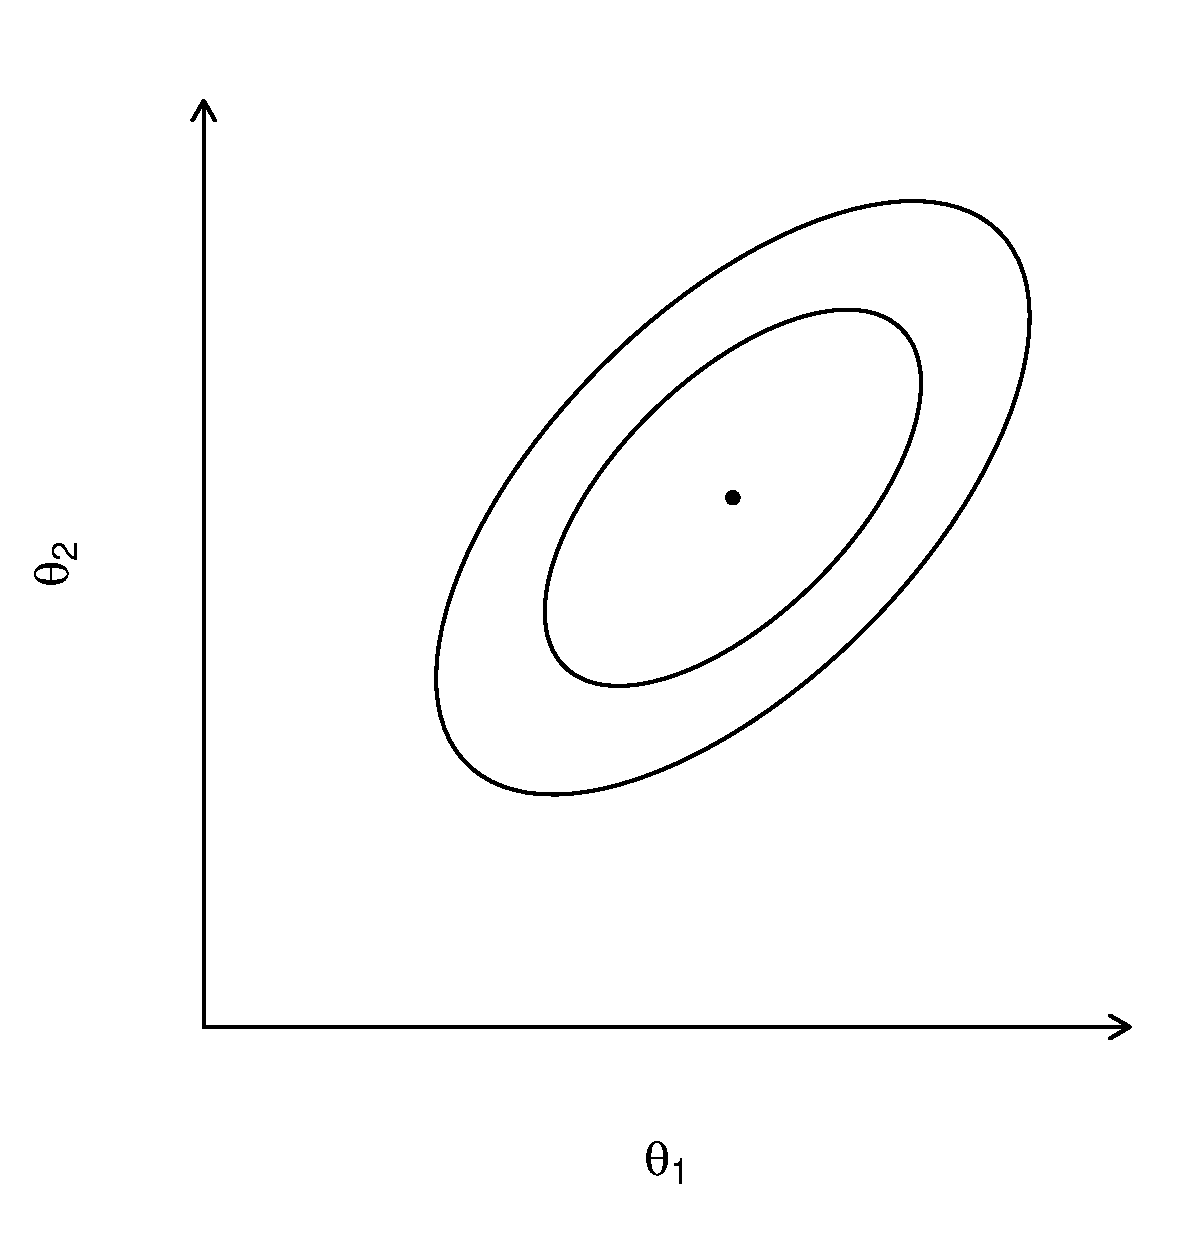
\includegraphics[width=5cm]{./graphics/ellipse1}
\end{itemize}
\end{frame}

\begin{frame}{1. More than one hyperparameter}
\protect\hypertarget{more-than-one-hyperparameter-1}{}
\textcolor{red}{Main use:} Select good evaluation points \({\theta}_k\)
for the numerical integration when approximating
\(\widetilde{\pi}(x_i|{y})\)

\begin{itemize}
\item
  Locate the mode
\item
  Compute the Hessian to construct principal components

  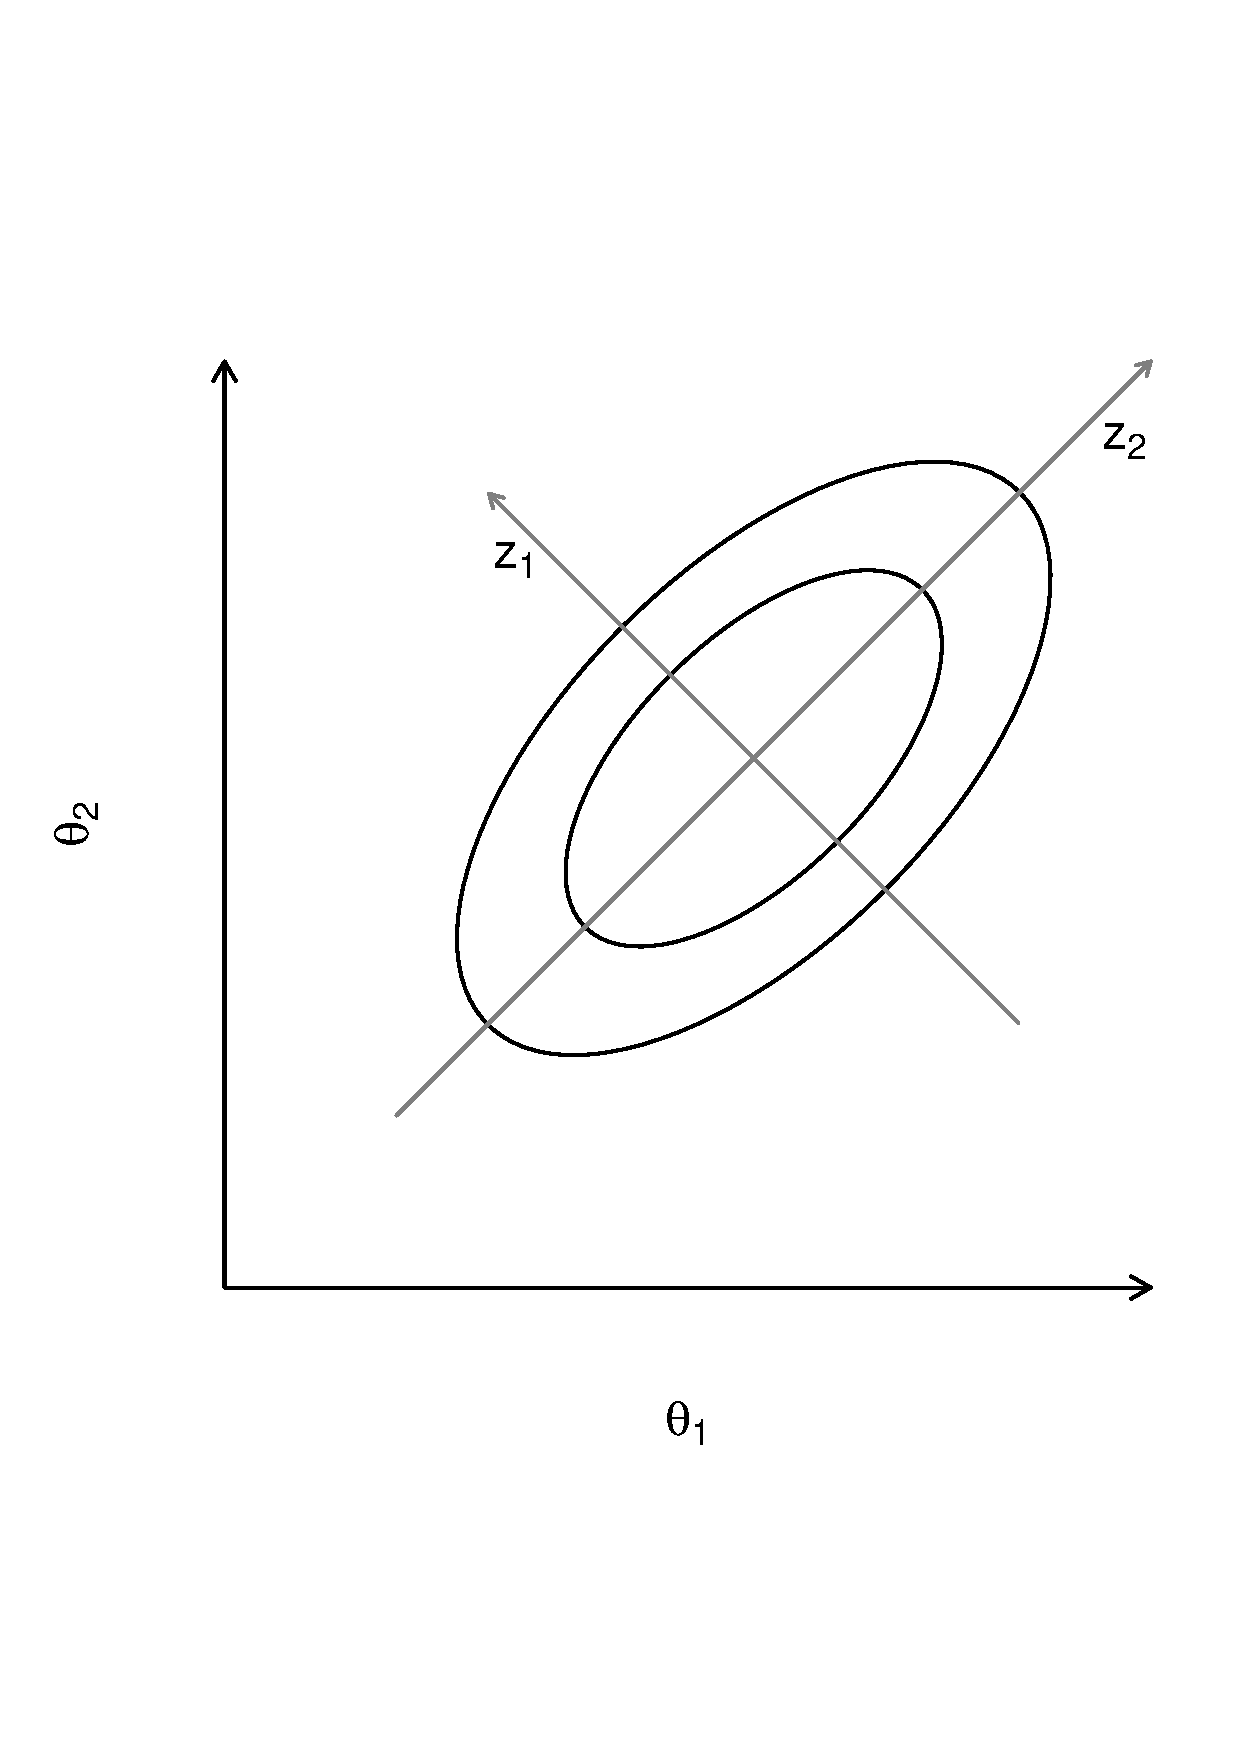
\includegraphics[width=5cm]{./graphics/ellipse2}
\end{itemize}
\end{frame}

\begin{frame}{1. More than one hyperparameter}
\protect\hypertarget{more-than-one-hyperparameter-2}{}
\textcolor{red}{Main use:} Select good evaluation points \({\theta}_k\)
for the numerical integration when approximating
\(\widetilde{\pi}(x_i|{y})\)

\begin{itemize}
\item
  Locate the mode
\item
  Compute the Hessian to construct principal components
\item
  Grid-search to locate bulk of the probability mass
  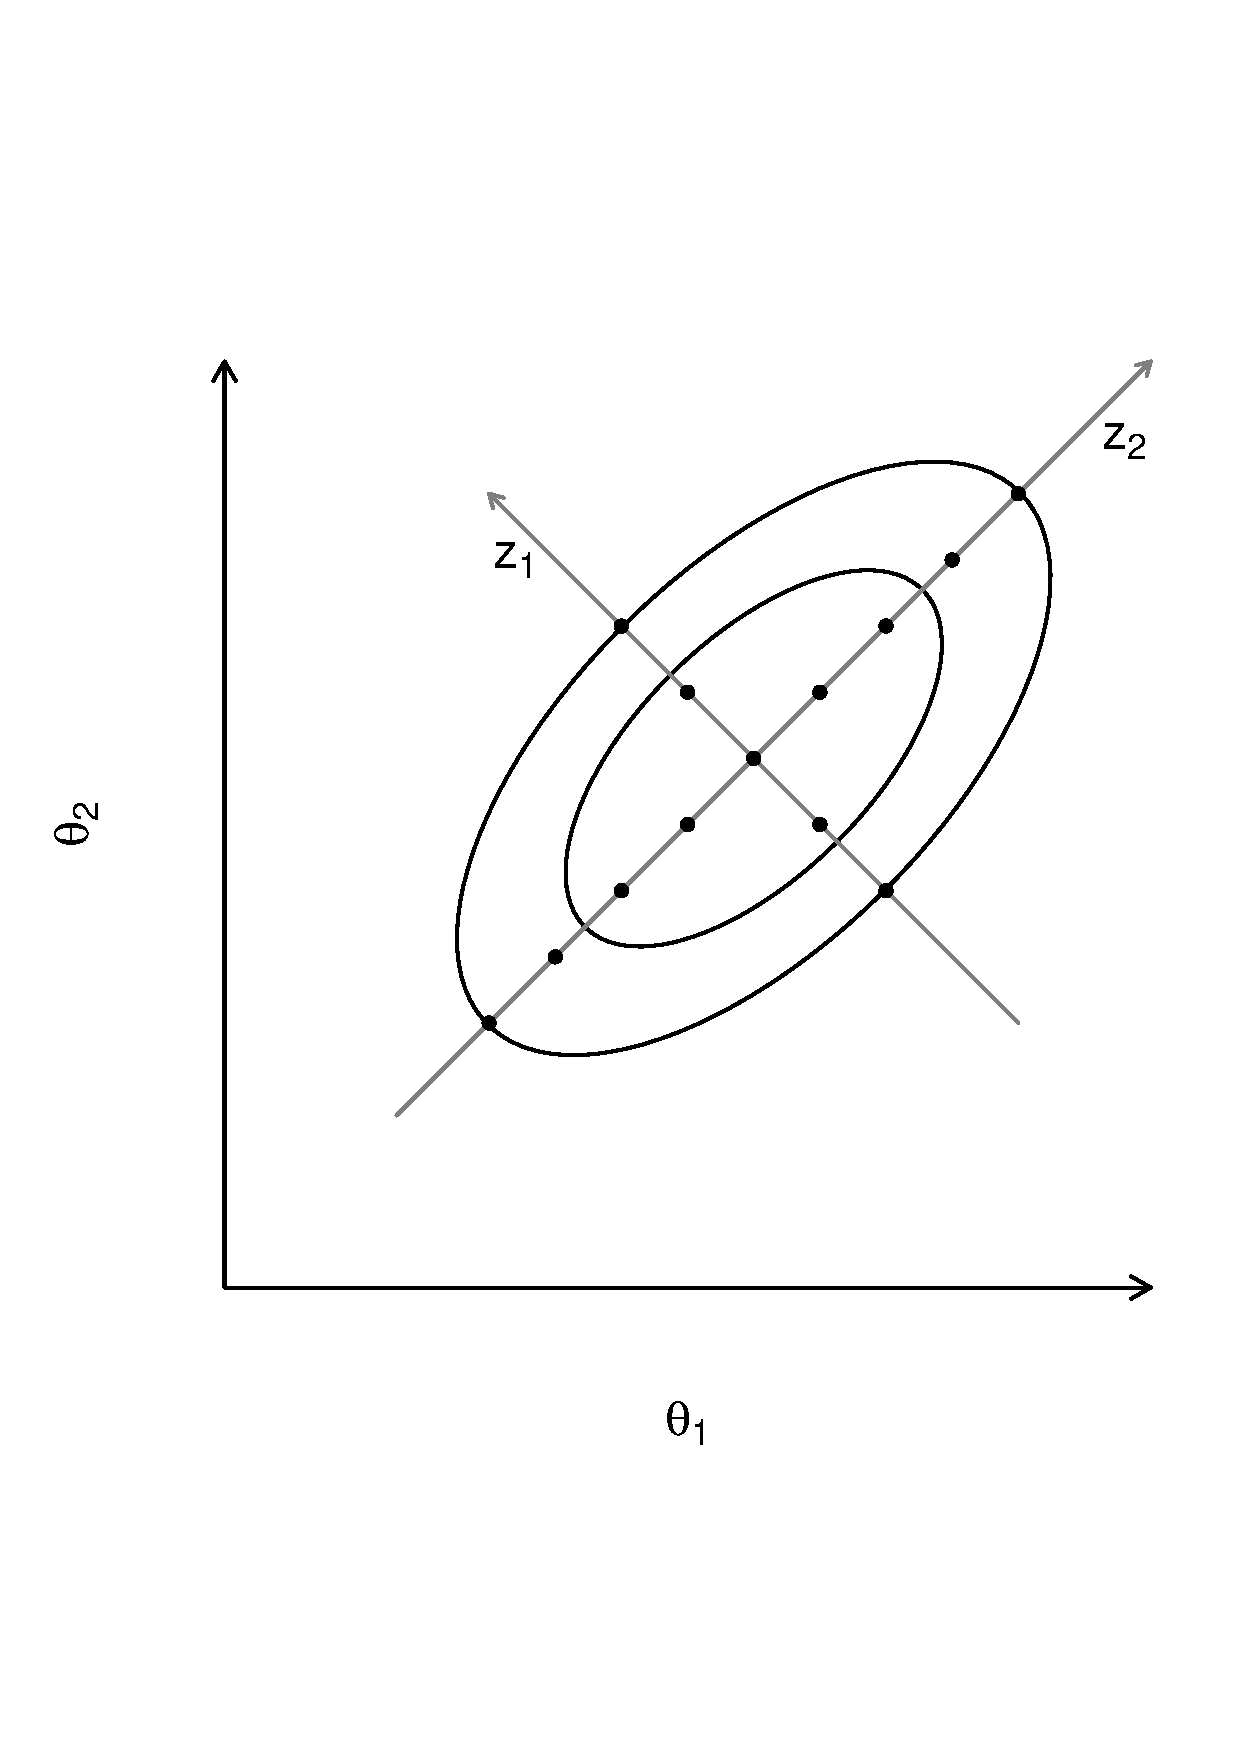
\includegraphics[width=5cm]{./graphics/ellipse3}
\end{itemize}
\end{frame}

\begin{frame}{1. More than one hyperparameter}
\protect\hypertarget{more-than-one-hyperparameter-3}{}
\begin{itemize}
\item
  Locate the mode
\item
  Compute the Hessian to construct principal components
\item
  Grid-search to locate bulk of the probability mass
\item
  For each point \(k\) in the grid compute:

  \begin{itemize}
  \tightlist
  \item
    \(\widetilde{\pi}(\theta^k|y)\)
  \item
    \(\widetilde{\pi}(x_i|\theta^k,y)\)
  \item
    \(\Delta_k\)
  \end{itemize}
\end{itemize}
\end{frame}

\begin{frame}{2. Non-Gaussian observations}
\protect\hypertarget{non-gaussian-observations}{}
In application we may choose likelihoods other than a Gaussian. How does
this change things?

\[
\pi(\mathbf{\theta} \mid \mathbf{y}) \propto \frac{
            \overbrace{\pi(\mathbf{x}, \mathbf{y}\mid \mathbf{\theta})}^{\text{Non-Gaussian, BUT KNOWN}}
        \; \pi(\mathbf{\theta})}{\underbrace{\pi(\mathbf{x} \mid \mathbf{y},
            \mathbf{\theta})}_{\text{Non-Gaussian and UNKNOWN}}}
\]

\begin{itemize}
\tightlist
\item
  In many cases
  \(\pi(\boldsymbol{x} \mid \boldsymbol{y}, \boldsymbol{\theta})\)is
  very close to a Gaussian distribution, and can be replaced with a
  \textcolor{red}{Laplace approximation}.
\end{itemize}
\end{frame}

\begin{frame}{The GMRF (Laplace) approximation}
\protect\hypertarget{the-gmrf-laplace-approximation}{}
Let \(\mathbf{x}\) denote a GMRF with precision matrix \(\mathbf{Q}\)
and mean \(\mathbf{\mu}\).

Approximate \[
\begin{aligned}
\pi(\mathbf{x}|\theta,\mathbf{y}) &\propto
            \exp\left(-\frac{1}{2}\mathbf{x}^\top \mathbf{Q}\mathbf{x} + \sum_{i=1}^n \log \pi (y_i|x_i)\right)
\end{aligned}
\] by using a second-order Taylor expansion of \(\log \pi (y_i|x_i)\)
around \(\mathbf{\mu}_0\), say.

\begin{itemize}
\tightlist
\item
  Recall \[
  \begin{aligned}
        f(x) \approx f(x_0) + f'(x_0)(x-x_0)+ \frac{1}{2} f''(x_0)(x-x_0)^2
        = a+ bx - \frac{1}{2}cx^2
  \end{aligned}
  \] with \[
  \begin{aligned}
  b &=f'(x_0) - f''(x_0)x_0\\
  c &= -f''(x_0)
  \end{aligned}
  \].
\end{itemize}

(Note: \(a\) is not relevant).
\end{frame}

\begin{frame}{The GMRF approximation (II)}
\protect\hypertarget{the-gmrf-approximation-ii}{}
Thus, \[
\begin{aligned}
        \widetilde{\pi}(\mathbf{x}|\mathbf{\theta}, \mathbf{y}) &\propto
            \exp\left(-\frac{1}{2}\mathbf{x}^\top \mathbf{Q}\mathbf{x}  +
            \sum_{i=1}^n (a_i + b_i x_i - 0.5 c_i x_i^2)\right)\\
        &{\propto \exp\left(-\frac{1}{2}\mathbf{x}^T(\mathbf{Q} + \text{diag}(\mathbf{c})) \mathbf{x} + \mathbf{b}^T\mathbf{x}\right)}
\end{aligned}
\]

which is Gaussian with precision matrix
\(\mathbf{Q} + \text{diag}(\mathbf{c})\) and mean given by the solution
of \((\mathbf{Q} + \text{diag}(\mathbf{c}))\mathbf{\mu} = \mathbf{b}\)

\textcolor{red}{The canonical parameterisation} is \[
\textcolor{red}{\mathcal{N}_C(\mathbf{b}, \mathbf{Q} + \text{diag}(\mathbf{c}))}
\] which corresponds to \[
\mathcal{N}((\mathbf{Q} + \text{diag}(\mathbf{c}))^{-1}\mathbf{b}, (\mathbf{Q} + \text{diag}(\mathbf{c}))^{-1}).
\]
\end{frame}

\begin{frame}{The GMFR approximation - One dimensional example}
\protect\hypertarget{the-gmfr-approximation---one-dimensional-example}{}
Assume \[
\begin{aligned}
  y|\lambda \sim\text{Poisson}(\lambda)  & \text{ Likelihood}\\
  \lambda = \exp(x)  & \text{ Likelihood}\\
  x\sim\mathcal{N}(0,1) & \text{ Latent Model}
\end{aligned}
\] we have that \[
  \pi(x|y)\propto\pi(y|x)\pi(x)\propto\exp\{ -\frac{1}{2}x^2+
  \underbrace{xy-\exp(x)}_{\text{non-gaussian part}}
  \}
\]
\end{frame}

\begin{frame}{The GMRF approximation}
\protect\hypertarget{the-gmrf-approximation}{}
\begin{center}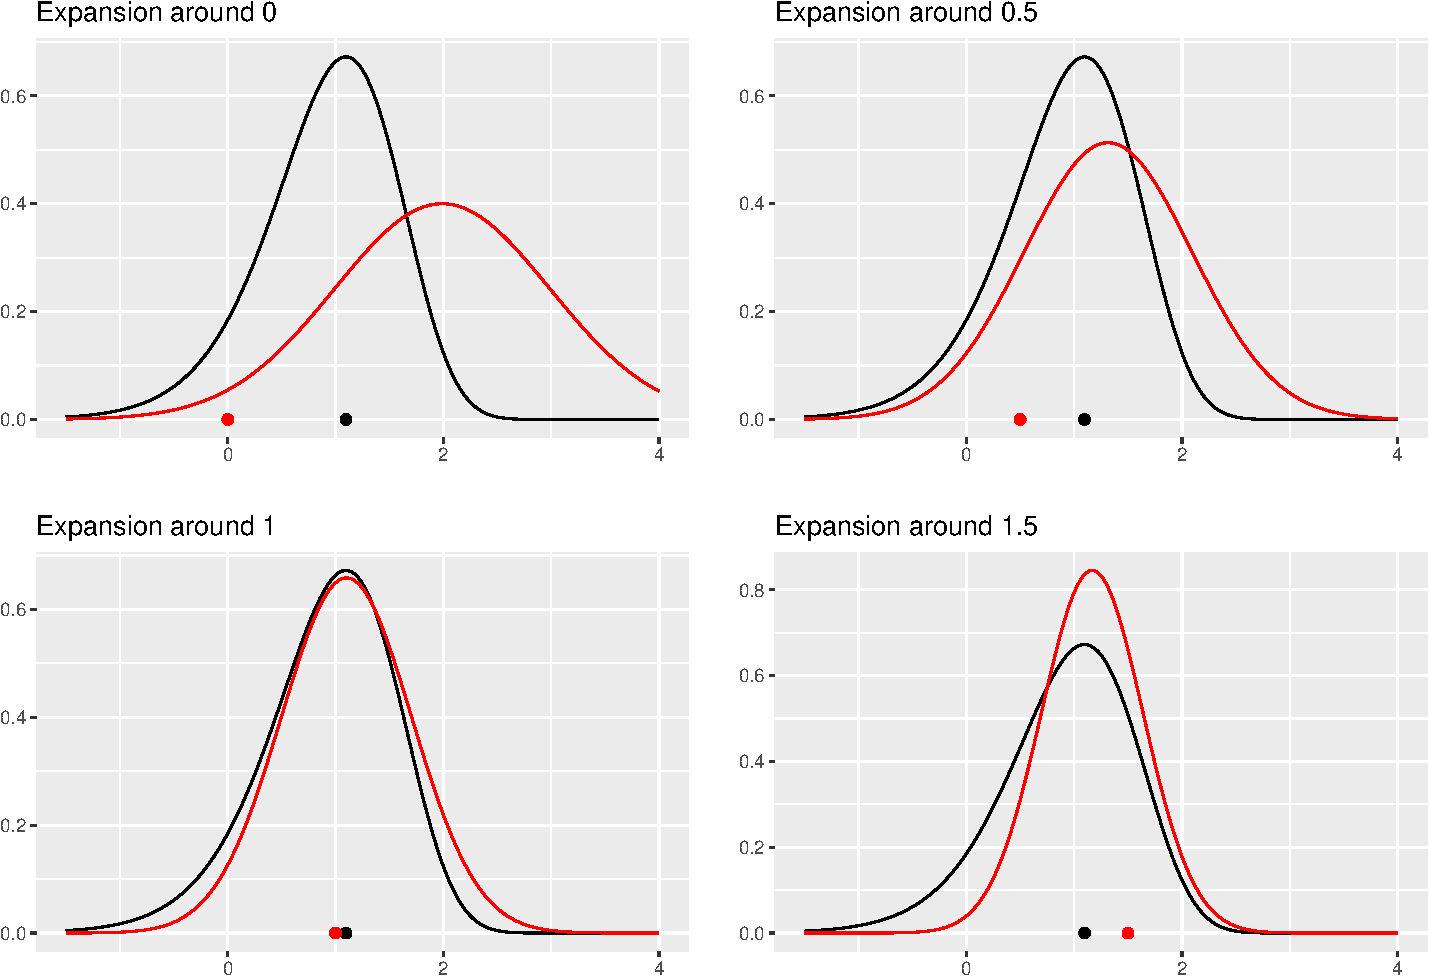
\includegraphics[width=0.6\linewidth]{Part2_deterministic_files/figure-beamer/unnamed-chunk-8-1} \end{center}

\textcolor{red}{If $\mathbf{y} \mid \mathbf{x}, \mathbf{\theta}$ is Gaussian "the approximation" is exact!}
\}
\end{frame}

\begin{frame}{What do we get \ldots{}}
\protect\hypertarget{what-do-we-get}{}
\[
\widetilde{\pi}(\mathbf{\theta} \mid \mathbf{y}) \propto  \frac{
           \pi(\mathbf{x}, \mathbf{y}\mid \mathbf{\theta})
        \; \pi(\mathbf{\theta})}{\widetilde{\pi}_G(\mathbf{x} \mid \mathbf{y},
            \mathbf{\theta})} \: \Bigg|_{\mathbf{x} = \mathbf{x}^\star(\mathbf{\theta})}
\]

\begin{itemize}
\item
  find the mode of \(\widetilde{\pi}(\mathbf{\theta}\mid \mathbf{y})\)
  (optimization)
\item
  explore \(\widetilde{\pi}(\mathbf{\theta}\mid \mathbf{y})\) to find
  grid points \(t_k\) for numerical integration.\\
  \strut \\
  \pause However, why is it called
  \textcolor{red}{integrated nested Laplace
      approximation}? \pause There is another step that changes: \[
  \pi(x_{i} \mid \mathbf{y}) \approx \sum_k \underbrace{\pi(x_{i} \mid \mathbf{y}, \theta^k)}_{{\text{Not Gaussian!}}}{\widetilde{\pi}_G(\theta^k\mid\mathbf{y})} \Delta_k
  \]
\end{itemize}
\end{frame}

\begin{frame}{Approximating \(\pi(x_i|\mathbf{y}, \mathbf{\theta})\)}
\protect\hypertarget{approximating-pix_imathbfy-mathbftheta}{}
Three possible approximations:

\begin{itemize}[<+->]
\item
  \begin{enumerate}[<+->]
  \tightlist
  \item
    \textcolor{red}{Gaussian distribution} derived from
    \(\widetilde{\pi}_G(\mathbf{x}|\mathbf{\theta}, \mathbf{y})\), i.e.
    \[
    \widetilde{\pi}(x_i|\mathbf{\theta}, \mathbf{y}) = \mathcal{N}(x_i; \mu_i(\mathbf{\theta}), \sigma_i^2(\mathbf{\theta}))
    \] with mean \(\mu_i(\mathbf{\theta})\) and marginal variance
    \(\sigma_i^2(\mathbf{\theta})\).\\
    However, errors in location and/or lack of skewness possible
  \end{enumerate}
\end{itemize}

\begin{itemize}[<+->]
\item
  \begin{enumerate}[<+->]
  \setcounter{enumi}{1}
  \tightlist
  \item
    \textcolor{red}{Laplace approximation}
  \end{enumerate}
\item
  \begin{enumerate}[<+->]
  \setcounter{enumi}{2}
  \tightlist
  \item
    \textcolor{red}{Simplified Laplace approximation}
  \end{enumerate}
\end{itemize}
\end{frame}

\begin{frame}{Laplace approximation of
\(\pi(x_i|\mathbf{\theta}, \mathbf{y})\)}
\protect\hypertarget{laplace-approximation-of-pix_imathbftheta-mathbfy}{}
Use again the same idea!

Based on the identity \[
\pi(z) = \frac{\pi(x,z)}{\pi(x|z)}\quad \text{ leading to }\quad \tilde{\pi}(z) = \frac{\pi(x,z)}{\tilde{\pi}(x|z)}\
\] When \(\tilde{\pi}(x|z)\) is the Gaussian approximation, this is the
Laplace approximation.
\end{frame}

\begin{frame}{Laplace approximation of
\(\pi(x_i|\mathbf{\theta}, \mathbf{y})\)}
\protect\hypertarget{laplace-approximation-of-pix_imathbftheta-mathbfy-1}{}
\[
\widetilde{\pi}_\text{LA}(x_i|\mathbf{\theta}, \mathbf{y}) \propto
            \frac{\pi(\mathbf{x}, \mathbf{\theta},\mathbf{y})}
            {\widetilde{\pi}_\text{GG}(\mathbf{x}_{-i}|x_i, \mathbf{\theta}, \mathbf{y})}
            \Biggr|_{\mathbf{x}_{-i}=\mathbf{x^\star}_{-i}(x_i, \mathbf{\theta})}
\]

The approximation is very good but expensive as \(n\) factorizations of
\((n-1) \times (n-1)\) matrices are required to get the \(n\) marginals.

\pause

\textcolor{blue}{Computational modifications exist:}

\begin{enumerate}
\tightlist
\item
  Approximate the modal configuration of the GMRF approximation.
\item
  Reduce the size \(n\) by only involving the ``neighbors'\,'.
\end{enumerate}
\end{frame}

\begin{frame}{Simplified Laplace approximation}
\protect\hypertarget{simplified-laplace-approximation}{}
Faster alternative to the Laplace approximation\\

\begin{itemize}
\tightlist
\item
  based on a \textcolor{red}{series
   expansion up to third order of the numerator and denominator of $\widetilde{\pi}_\text{LA}(x_i|\mathbf{\theta}, \mathbf{y})$}
\item
  corrects the Gaussian approximation for error in location and lack of
  skewness.
\end{itemize}

\pause

This is \textcolor{red}{default option when using INLA} but this choice
can be modified.
\end{frame}

\begin{frame}{INLA: When does it work}
\protect\hypertarget{inla-when-does-it-work}{}
We consider models of the kind \[
\begin{aligned}
\theta & \sim \pi(\theta)\\
\mathbf{x}|\theta& \sim \pi(\mathbf{x}|\theta) = \mathcal{N}(0, \mathbf{Q}^{-1}(\theta))\\
\mathbf{y}|\mathbf{x},\theta & \sim \prod_i\pi(y_i|\eta_i,\theta)
\end{aligned}
\] where

\begin{itemize}
\item
  \(\mathbf{x}\) can be large but endowed with Markov properties so that
  \(\mathbf{Q}(\theta)\) is sparse
\item
  the size of \(\theta\) is small (say \textless15)
\item
  \(\eta\) is a predictor that depends \emph{linearly} on the other
  elemets of \(\mathbf{x}\)
\item
  The main inferential interest lies in the posterior marginals
  \(\pi(x_i|\mathbf{y})\), \(\pi(\theta_j|\mathbf{y})\) rather than in
  the joint \(\pi(\mathbf{x},\theta|\mathbf{y})\) (\ldots.but joint
  inference is possible through sampling!)
\end{itemize}
\end{frame}

\begin{frame}{INLA: Overview}
\protect\hypertarget{inla-overview}{}
\begin{itemize}
\item
  \textbf{Step I} Approximate \(\pi({\theta}|y)\) using the Laplace
  approximation and select good evaluation points \({\theta}_k\).
\item
  \textbf{Step II} For each \({\theta}_k\) and \(i\) approximate
  \(\pi(x_i|{\theta}_k, {y})\) using the Laplace or simplified Laplace
  approximation for selected values of \(x_i\)
\item
  \textbf{Step III} For each \(i\), sum out \({\theta}_k\) \[
  \widetilde{\pi}(x_i|{y}) = \sum_k \widetilde{\pi}(x_i|{\theta}_k, {y}) \times
                    \widetilde{\pi}({\theta}_k|{y}) \times \Delta_k.
  \] Build a log spline corrected Gaussian to represent
  \(\widetilde{\pi}(x_i|{y})\).
\end{itemize}
\end{frame}

\begin{frame}{INLA: Why does it work?}
\protect\hypertarget{inla-why-does-it-work}{}
\begin{itemize}
\item
  The full conditional \(\pi(x|y,\theta)\) is ``almost'' Gaussian
\item
  The latent field \(x\) is a GMRF

  \begin{itemize}
  \tightlist
  \item
    GMRF \(\rightarrow\) sparse precision matrix!!
  \item
    Easy to solve and store
  \end{itemize}
\item
  Smart numerical methods
\item
  Parallel implementation
\end{itemize}
\end{frame}

\begin{frame}{Limitations}
\protect\hypertarget{limitations}{}
\begin{itemize}
\item
  The dimension of the latent field \(x\) can be large (\(10^2-10^6\))
\item
  The dimension of the hyperparameters \(\theta\) must be small
  (\(\leq 9\))
\end{itemize}

In other words, each random effect can be big, but there cannot be too
many random effects unless they share parameters.
\end{frame}

\begin{frame}{INLA: summary}
\protect\hypertarget{inla-summary}{}
\begin{itemize}
\item
  These are the basic ideas
\item
  The rest are \emph{just} details\ldots.but there are a lot of them!
\end{itemize}
\end{frame}

\begin{frame}{INLA features}
\protect\hypertarget{inla-features}{}
INLA fully incorporates posterior uncertainty with respect to
hyperparameters \(\Rightarrow\) tool for full Bayesian inference

\begin{itemize}
\tightlist
\item
  Marginal posterior densities of all (hyper-)parameters
\item
  Posterior mean, median, quantiles, std.\textasciitilde deviation, etc.
\item
  The approach can be used for predictions, model assessment, \ldots
\item
  Joint posterior marginal not available\ldots but it is possible to
  sample from \(\widetilde{\pi}(x,\theta|y)\)
\end{itemize}
\end{frame}

\end{document}
